\documentclass[./../../paper.tex]{subfiles}
\graphicspath{{\subfix{./../../figures/}}}

\begin{document}

\section{Determine the Evolutionary Algorithm Configurations}

\subsection{Experimental Setup}
\label{sec:exp1}
As explained in \autoref{sec:evolutionary}, there are many possible configurations for an evolutionary algorithm. Therefore, we test combinations of all mentioned configurations for each phase of our evolutionary algorithm. 

The combinatory set of all phase options contains \attention{144} elements. To avoid confusion, we refer to each unique phase combination as a configuration. We choose to run each configuration for \attention{50} evolution cycles. For all configurations we use the same set of \attention{5} factual \glspl{instance}, which are randomly sampled from the validation set. We decide to return \attention{500} survivors at the end of each run for every factual case. The initiation phase samples \attention{1000} initial individuals for the population \optional{EXCEPT FittestInitiator, REASON}. Within each cycle, we generate \attention{2000} new offsprings. And choose to add \attention{500} individuals to the population\attention{Revise in code and text}. We keep the mutation rate uniform. Hence, we each delete, insert, change and transpose approximately \attention{20\%} mutation phase. The remaining \attention{20\%} we do not apply any change. We apply each edit-type by a constant edit-rate of \attention{10\%} of the sequence length. 

After retrieving the results, we fit a linear mixed-effects model to determine the importance of each configuration. Here, we use the resulting viability as a dependent variable and each phase as independent variable. We adjust the model according to their configuration, as we retrieve \attention{50} samples per configuration. If a phase-type strongly affects the dependent variable and the resulting change is deemed significant, we can draw conclusions about the full configuration. Furthermore, preliminary results showed that many of the configurations have a zero feasibility. Hence, we also incorporate the insights gained from using feasibility as a dependent variable.

\subsection{Results}

% TODO: Change plots to matplotlib plots
\begin{figure}
    \centering
    \begin{subfigure}[c]{0.99\textwidth}
        \centering
        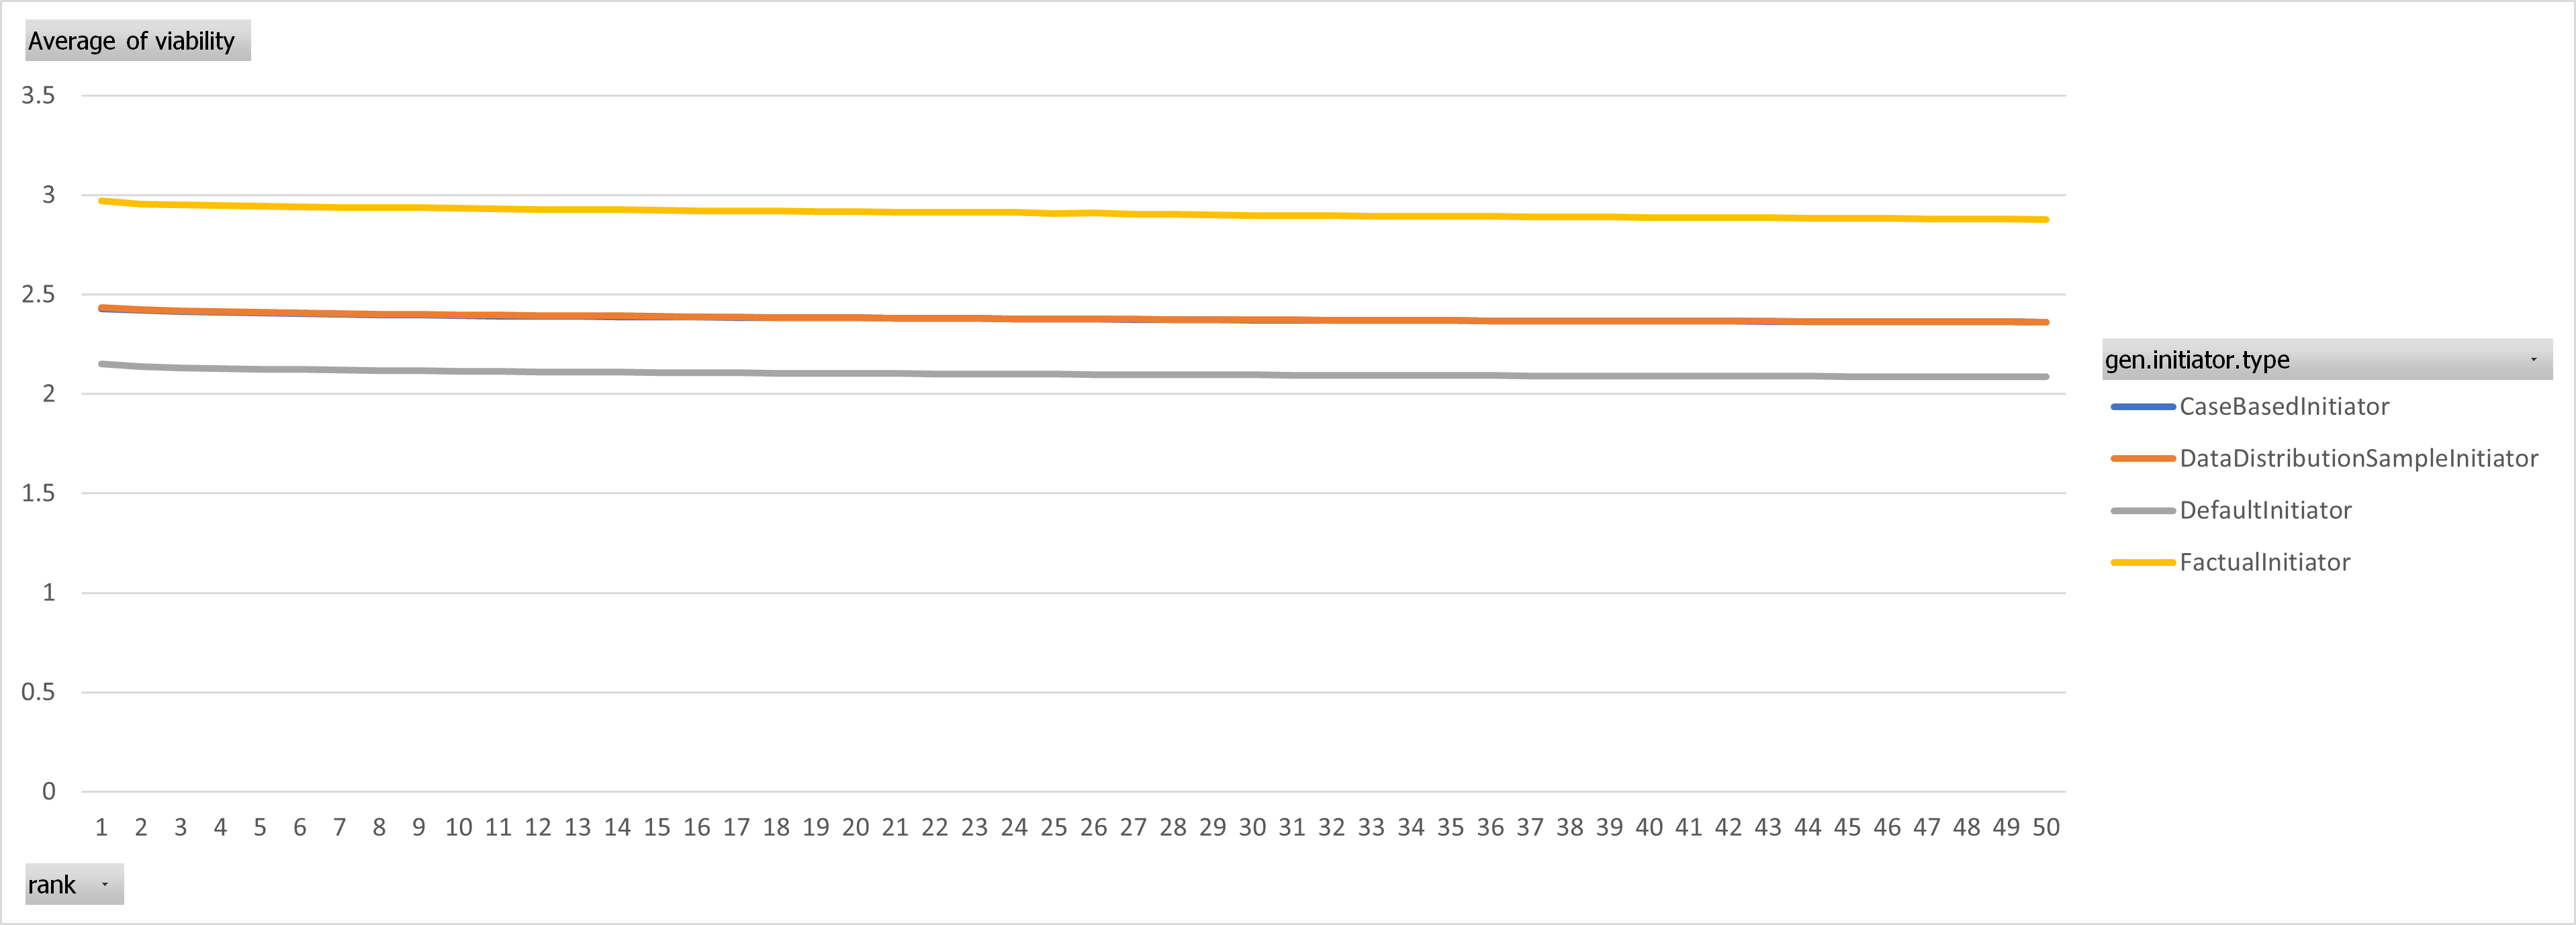
\includegraphics[width=\textwidth]{figures/plots/average_viability.png}
        \caption{This figure shows the average viability of the 50 best counterfactuals for each configuration. The x-axis shows their respective rank.}
        \label{fig:average_viability}
    \end{subfigure}
    \begin{subfigure}[c]{0.99\textwidth}
        \centering
        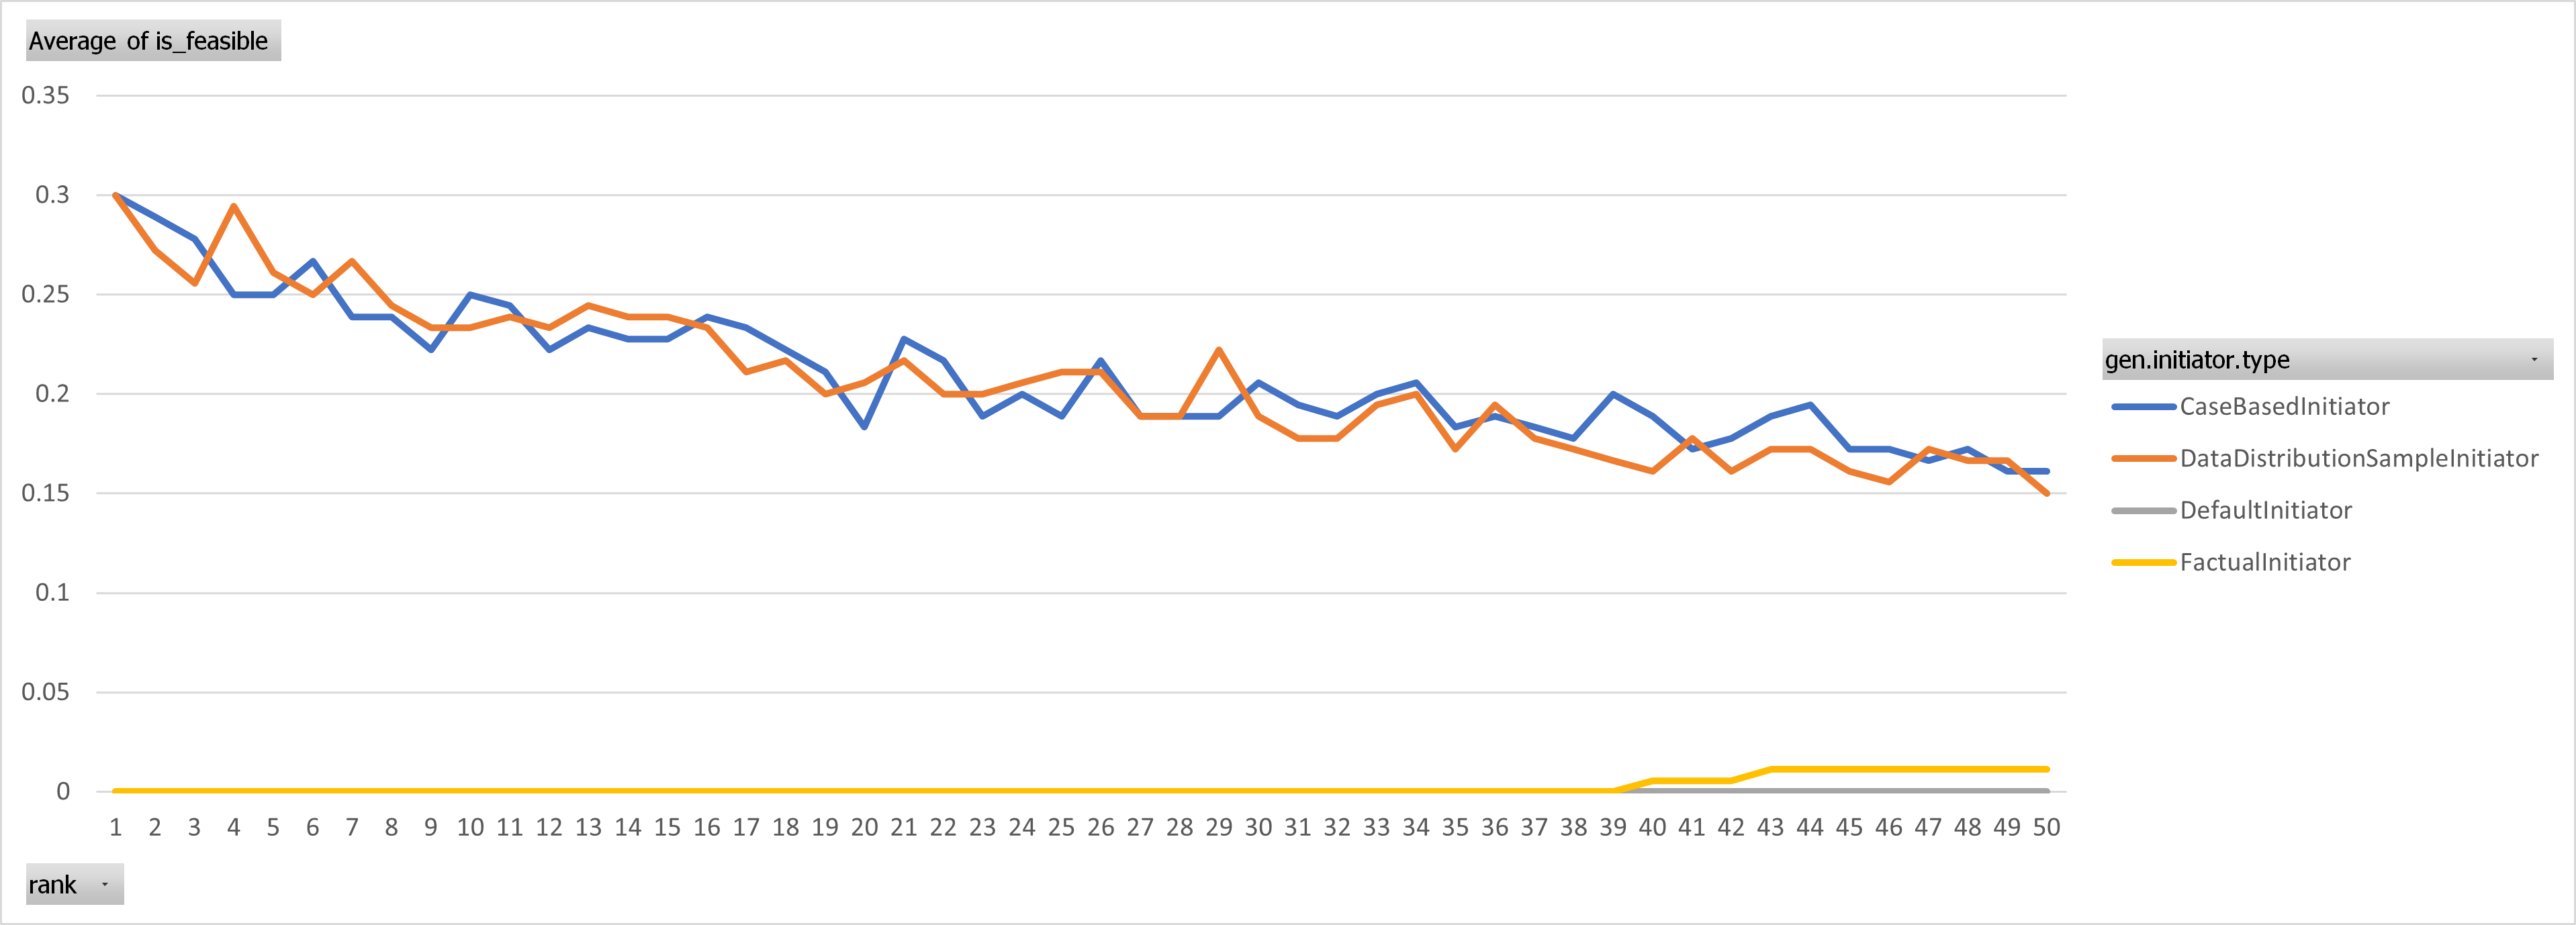
\includegraphics[width=\textwidth]{figures/plots/average_feasibility.png}
        \caption{This figure shows the average feasibility of the 50 best counterfactuals for each configuration. The x-axis shows their respective rank.}
        \label{fig:average_feasibility}
    \end{subfigure}
\end{figure}


\needstbl{tbl:viability}{This table shows the results of the mixed linear model using viability as dependent variable.}

\needstbl{tbl:feasibility}{This table shows the results of the mixed linear model using feasibility as dependent variable.}

In terms of viability, we see that the factual initiator is clearly superior. However, the results for using the factual itself are nearly identical.  \attention{0.2\%} of the counterfactuals generated with this inititator resulted in a feasibility non-zero probability. In contrast, for the  \attention{CBS and DDS} initiators the fraction of non-zero probability counterfactuals is \attention{20.9\%} and \attention{20.7\%} respectively. If we consider the ranks of each constructed counterfactual per configuration we see a clear difference between \attention{CBI and DDI} opposed to \attention{FI}. It does not surprise, that the \attention{DI} fails to generate any feasible counterfactual across all configurations. If we consider the mixed-effects linear model, we see a similar pattern emerging. We see that the effect of the \attention{FI} is significant for both, the viability and the feasibility. However, the effect is positive and negative, respectively. 

\subsection{Discussion}
Whether these values are the theoretical ceiling, requires further investigations. However, the reasons for this behavior are clear. If we start the model with the factuals as initial population, the factual will already have a viability of at least 2 as similiarity and sparcity have to be at their maximal value. As the prediction model tends only assign scores close to the extremes, the favorable change of an event attribute often yields a strong improvement in likelihood. Hence, the viabilities often reach a viability of 3. The only way to reach higher viability values is to approach the pareto-surface by changing the feasibility. In other words, we have to increase feasibility without significantly decreasing the scores for similarity, sparcity and the improvement. 

Moving forward, we have to choose a set of configurations and also determine suitable hyperparameters for each. In the next experiment we consider \attention{a couple of configuration phases}.  

\end{document}